\section{Самофокусировки пучков с регулярной поперечной структурой}
\label{sec:beams}

\subsection{Постановка задачи}

В данной главе рассматривается самофокусировка неограниченных пучков, описываемых формулами:

\begin{align}
    \label{BeamsInfinityInitialOutphase}
    E(x, y, z = 0) & = \cos(\alpha_m x) \cos(\alpha_m y) \\
    \label{BeamsInfinityInitialInphase}
    E(x, y, z = 0) & = \left| \cos(\alpha_m x) \cos(\alpha_m y) \right|
\end{align}

Коэффициент $\alpha_m$ в этих формулах задаётся таким образом, чтобы на полуширине расчётной области
укладывалось $m$ периодов косинуса, что понадобится для согласования граничных условий при моделировании
неограниченных пучков c периодической поперечной структурой:

\begin{equation}
    \alpha_m = \frac{2\pi}{L} m
\end{equation}

Далее рассматривается процесс филаментации структурированных пучков с гауссовским поперечным профилем, описываемых формулами:

\begin{align}
    \label{BeamsGaussInitialOutphase}
    E(x, y, z = 0) & = \exp \left( -\frac{x^2 + y^2}{2 a^2}\right) \cos(\alpha_m x) \cos(\alpha_m y) \\
    \label{BeamsGaussInitialInphase}
    E(x, y, z = 0) & = \exp \left( -\frac{x^2 + y^2}{2 a^2}\right) \left| \cos(\alpha_m x) \cos(\alpha_m y) \right|
\end{align}

Пучки вида (\ref{BeamsInfinityInitialOutphase}) и (\ref{BeamsGaussInitialOutphase}) будем условно называть противофазными,
так как в~соседних пичках импульса фаза волны отличается на $\pi$,
а пучки вида (\ref{BeamsInfinityInitialInphase}) и (\ref{BeamsGaussInitialInphase}) "--- синфазными,
так как фаза пучка одинакова во всех точках поперечного сечения пучка.


В данной задаче исследовался начальный этап филаментации, что позволило учитывать в вычислениях
только дифракцию по пространству и керровскую нелинейность.


\subsection{Самофокусировка неограниченных пучков}

Как было показано в гл. \ref{sec:model}, алгоритм, использующий БПФ, применим для исследования
распространения бесконечно-широких поперечно-периодичных пучков. Единственное, о~чём нужно помнить,
это равенство граничных условий на противоположных сторонах выбранной расчётной области.


В качестве рассматриваемой области был выбран квадрат, а поле описывалось
формулами~(\ref{BeamsInfinityInitialOutphase})--(\ref{BeamsInfinityInitialInphase}) при значении $m = 1$.

%%%%%%%%%%%%%%%%%%%%%%%%%%%%%%%%%%%%%%%%

\begin{figure}[H]
    \begin{center}
        \begin{minipage}{\minipagewidththree}
            \center{\includegraphics[width=0.95\linewidth]{beams/infinity/out00000_norm} \\
            \footnotesize{$z = 0.00$}}
        \end{minipage}
        \hspace{\minipagewidthpadding}
        \begin{minipage}{\minipagewidththree}
            \center{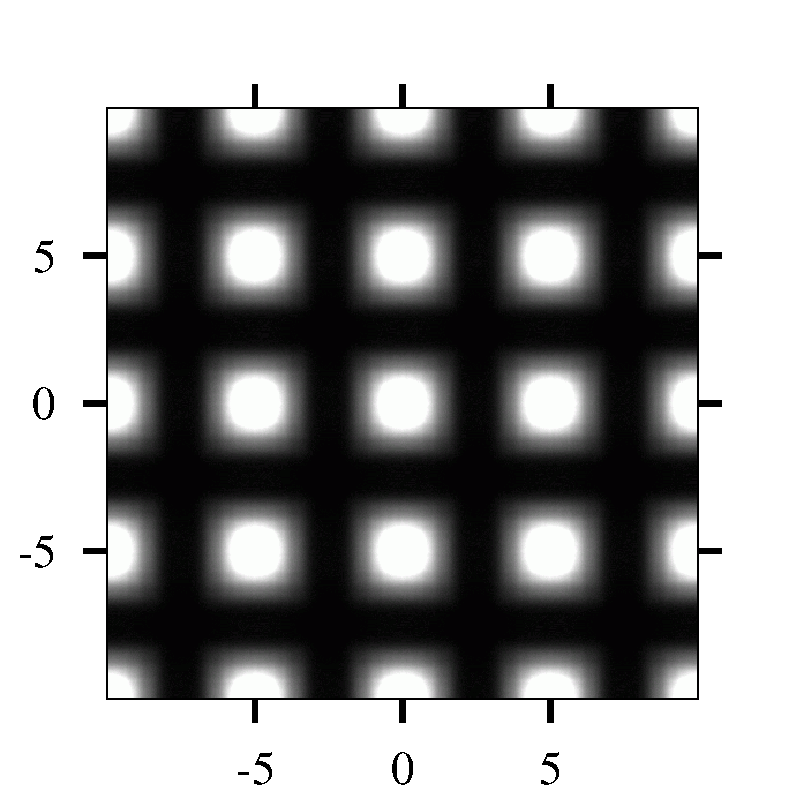
\includegraphics[width=0.95\linewidth]{beams/infinity/out00080_norm} \\
            \footnotesize{$z = 0.105$}}
        \end{minipage}
        \\
        \begin{minipage}{\minipagewidththree}
            \center{\includegraphics[width=0.95\linewidth]{beams/infinity/out00100_norm} \\
            \footnotesize{$z = 0.117$}}
        \end{minipage}
        \hspace{\minipagewidthpadding}
        \begin{minipage}{\minipagewidththree}
            \center{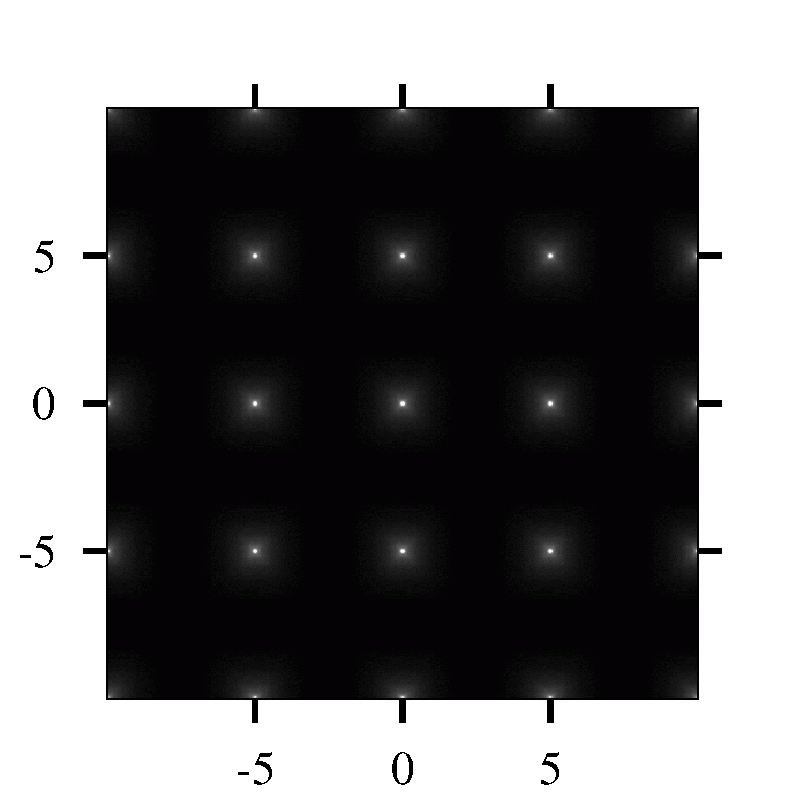
\includegraphics[width=0.95\linewidth]{beams/infinity/out00140_norm} \\
            \footnotesize{$z = 0.126$}}
        \end{minipage}
        \\[1ex]
        \caption{Начальное распределение и процесс самофокусировки отдельных пичков неограниченного синфазного пучка. $R = 100 \simeq R_{cr}$.}
        \label{fig:BeamsInfinityOutphase}
    \end{center}
\end{figure}

%%%%%%%%%%%%%%%%%%%%%%%%%%%%%%%%%%%%%%%%

Если в среде присутствует нелинейность, то каждый из пичков подвергается самофокусировке, что видно на рис. \ref{fig:BeamsInfinityOutphase}.
По формуле Марбургера с $R_{cr}^{Gauss}$ для гауссового пучка, $R = 100$ было получено расстояние филаментации,
равное $0.095$, но~в~численном расчёте на~этом расстоянии интенсивность не~превысила начальную и~в~два~раза. 
Это можно связать с~тем, что из-за близости филаментов они взаимодействуют друг~с~другом, отдаляя точку возникновения филамента,
а~также с~изменением величины $R_{cr}$ вследствии изменения формы пучка.

%%%%%%%%%%%%%%%%%%%%%%%%%%%%%%%%%%%%%%%%

\begin{figure}[H]
    \begin{center}
        \begin{minipage}{\minipagewidthtwo}
            \center{\includegraphics[width=0.95\linewidth]{beams/infinity/graph}}
        \end{minipage}
       \\[1ex]
        \caption{Увеличение пиковой интенсивности неограниченного пучка с регулярной поперечной структурой при приближении к нелинейному фокусу.
                 Вертикальные линии соответствуют расстояниям, распределения интенсивности на которых показаны на рис.  \ref{fig:BeamsInfinityOutphase}.}
        \label{fig:BeamsInfinityIz}
    \end{center}
\end{figure}

%%%%%%%%%%%%%%%%%%%%%%%%%%%%%%%%%%%%%%%%

Если рассматривать синфазный пучок, описываемый формулой (\ref{BeamsInfinityInitialInphase}), то~процесс возникновения
филаментов при такой же мощности практически не отличается от противофазного случая.
Скорее всего это связано не с особенностями модуляции, а~с~дефектом метода из-за того,
что в синфазном случае есть излом в амплитуде поля, который приводит к большой ширине спектра,
а значит не совсем корректным использование дискретного преобразования Фурье для решения уравнения дифракции.


\subsection{Самофокусировка ограниченных пучков с гауссовским поперечным профилем}

Понятно, что довольно сложно создать периодическую структуру с шириной, достаточной для того, чтобы считать пучок <<бесконечным>>.
Намного проще сделать ограниченный пучок, соответствующий формулам (\ref{BeamsGaussInitialOutphase}) и (\ref{BeamsGaussInitialInphase}).
Рассмотрим, как распространяется подобный пучок в среде с керровской нелинейностью,
будут ли возникать филаменты и как периодическая структура пучка влияет на процесс образования филамента.


Для исследования распространения импульса на большие расстояния и для уменьшения эффекта <<отражения>> импульса
от границ расчётной области (следствие применения дискретного преобразования Фурье) полуширина области выбиралась равной десяти радиусам
огибающей импульса, $L = 10$. Число периодов косинуса на полуширину окна $m = 16$,
а~значит в формулах (\ref{BeamsGaussInitialOutphase})-(\ref{BeamsGaussInitialInphase}) $\alpha = \alpha_{16} = 2 \pi \frac{16}{10}$.


Попробуем оценить критическое значение параметра $R$ для такого пучка. Прямым интегрированием можно показать, что при одинаковой
пиковой интенсивности энергия пучка с регулярной поперечной структурой почти в 4 раза меньше, чем энергия пучка с гауссовой огибающей такого же радиуса:

\begin{equation}
\left. \frac{W}{W_{\alpha}} \right|_{\alpha = \alpha_{16}} = \left. 4 \frac{e^{2\alpha^2}}{(e^{\alpha^2} + 1)^2} \right|_{\alpha = \alpha_{16}} \approx 4.
\end{equation}

Это означает, что можно ожидать $R_{cr}^{*} \approx 15$. Однако, в случае противофазных возмущений (\ref{BeamsGaussInitialOutphase})
вычислительный эксперимент даёт следующий результат:
за~счёт дифракции структура начинает расплываться от центра импульса вследствие асимметрии пиков структуры.
В результате этого процесса возникают четыре области концентрации энергии, разбегающиеся
от начала координат в стороны. Возникновение именно четырёх пучков связано с геометрией задачи.
Таким образом, критической значение необходимо увеличить в 4 раза:  $R_{cr}^{outphase} = R_{cr}^{gauss} \cdot 4 \cdot 4 = 60.3$.

%%%%%%%%%%%%%%%%%%%%%%%%%%%%%%%%%%%%%%%%

\begin{figure}[H]
    \begin{center}
        \begin{minipage}{\minipagewidththree}
            \center{\includegraphics[width=0.95\linewidth]{beams/r_0_outphase/out00000_norm} \\[0.1ex]
            \footnotesize{$z = 0$ }}
        \end{minipage}
        \hfill
        \begin{minipage}{\minipagewidththree}
            \center{\includegraphics[width=0.95\linewidth]{beams/r_0_outphase/out00010_norm} \\[0.1ex]
            \footnotesize{$z = 0.1$}}
        \end{minipage}
        \hfill
        \begin{minipage}{\minipagewidththree}
            \center{\includegraphics[width=0.95\linewidth]{beams/r_0_outphase/out00020_norm} \\[0.1ex]
            \footnotesize{$z = 0.2$}}
        \end{minipage}
       \\[0.5ex]
        \begin{minipage}{\minipagewidththree}
            \center{\includegraphics[width=0.95\linewidth]{beams/r_0_outphase/out00030_norm} \\[0.1ex]
            \footnotesize{$z = 0.3$ }}
        \end{minipage}
        \hfill
        \begin{minipage}{\minipagewidththree}
            \center{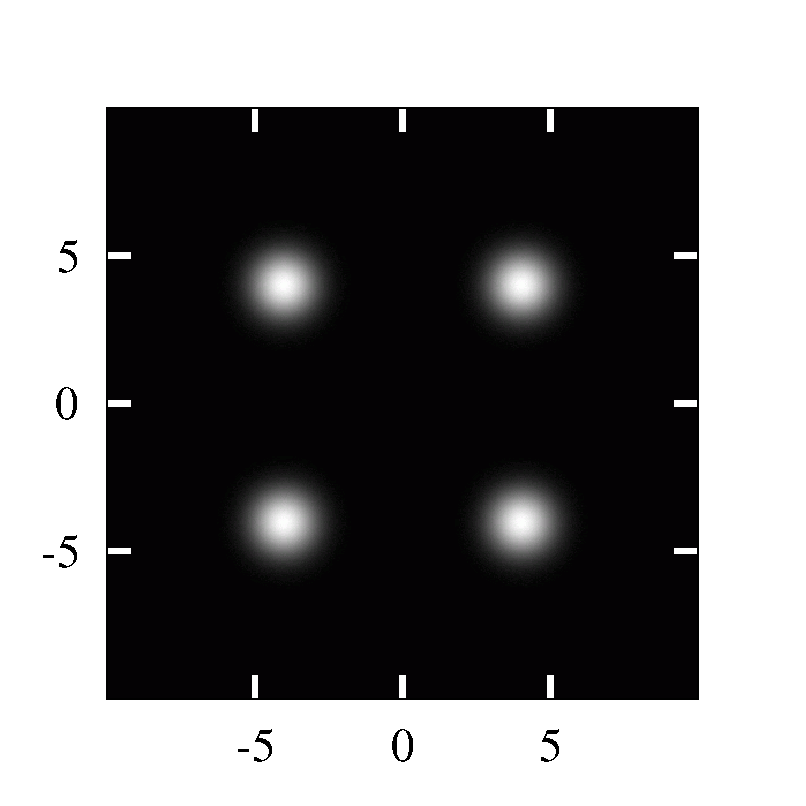
\includegraphics[width=0.95\linewidth]{beams/r_0_outphase/out00040_norm} \\[0.1ex]
            \footnotesize{$z = 0.4$}}
        \end{minipage}
        \hfill
        \begin{minipage}{\minipagewidththree}
            \center{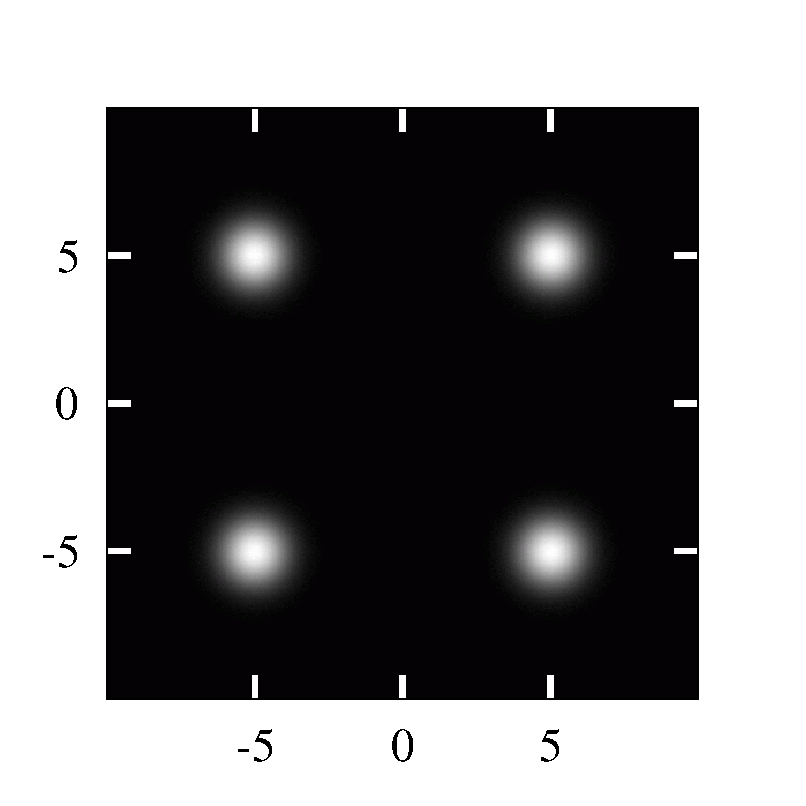
\includegraphics[width=0.95\linewidth]{beams/r_0_outphase/out00050_norm} \\[0.1ex]
            \footnotesize{$z = 0.5$}}
        \end{minipage}
       \\[0.6ex]
        \caption{Процесс распада противофазного пучка на четыре в случае отсутствия нелинейности. \\
                 Начальное распределение для наглядности показано в увеличенном виде.}
        \label{fig:BeamsR0outphase}
        \vspace{1ex}
        \begin{minipage}{\minipagewidththree}
            \center{\includegraphics[width=0.95\linewidth]{beams/r_100_outphase/out00000_norm} \\[0.1ex]
            \footnotesize{$z = 0$ }}
        \end{minipage}
        \hfill
        \begin{minipage}{\minipagewidththree}
            \center{\includegraphics[width=0.95\linewidth]{beams/r_100_outphase/out00100_norm} \\[0.1ex]
            \footnotesize{$z = 0.1$}}
        \end{minipage}
        \hfill
        \begin{minipage}{\minipagewidththree}
            \center{\includegraphics[width=0.95\linewidth]{beams/r_100_outphase/out00200_norm} \\[0.1ex]
            \footnotesize{$z = 0.2$}}
        \end{minipage}
       \\[0.5ex]
        \begin{minipage}{\minipagewidththree}
            \center{\includegraphics[width=0.95\linewidth]{beams/r_100_outphase/out00300_norm} \\[0.1ex]
            \footnotesize{$z = 0.3$ }}
        \end{minipage}
        \hfill
        \begin{minipage}{\minipagewidththree}
            \center{\includegraphics[width=0.95\linewidth]{beams/r_100_outphase/out00400_norm} \\[0.1ex]
            \footnotesize{$z = 0.4$}}
        \end{minipage}
        \hfill
        \begin{minipage}{\minipagewidththree}
            \center{\includegraphics[width=0.95\linewidth]{beams/r_100_outphase/out00500_norm} \\[0.1ex]
            \footnotesize{$z = 0.5$}}
        \end{minipage}
       \\[0.5ex]
        \caption{Процесс образования филаментов при $R = 100$ в случае противофазно модулированного пучка.
                 Начальное распределение для наглядности показано в увеличенном виде.}
        \label{fig:BeamsR100outphase}
    \end{center}
\end{figure}

%%%%%%%%%%%%%%%%%%%%%%%%%%%%%%%%%%%%%%%%

В случае, если мощности импульса не хватает для возникновение четырёх филаментов
(рис. \ref{fig:BeamsR0outphase}), пички убегают от начала координат,
испытывая дифракционную расходимость.

Как видно из рис. \ref{fig:BeamsR0outphase}--\ref{fig:BeamsR100outphase}, образование четырёх пучков либо филаментов
связано с дифракцией начального распределения на начальном этапе распространения. На~основе полученных данных были рассчитаны
величины расхождения пучков для приведённых случаев без нелинейности и при $R = 100$. Характерный диаметр исходного
пучка $a = 1\text{см}$, длина волны $\lambda = 800\text{нм}$. Отсюда $z_d = k a^2 = \frac{2\pi}{\lambda} a^2 = 785\text{м}$.
В~соответствии с приведёнными выше данными для $R = 100$ при $\tilde{z} = 0.5$ получим $z = 392\text{м}$, а~расстояние между пучками
$\Delta_{R = 0} \simeq 5.0\text{см}$ и $\Delta_{R = 100} \simeq 4.9\text{см}$. Таким образом, для прогнозирования
положения филаментов можно воспользоваться линейным уравнением, решение которого с помощью метода на основе преобразования Фурье можно
получить для любого $z$ за один шаг, так как различие между положениями максимумов в~линейном и нелинейном случаях
составляют всего несколько процентов.

\begin{figure}[h!]
    \begin{center}
        \begin{minipage}{\minipagewidthtwo}
            \center{\includegraphics[width=0.95\linewidth]{beams/marburger/graph_outphase}}
        \end{minipage}
       \\[1ex]
        \caption{Зависимость расстояния до нелинейного фокуса от параметра нелинейности $R$ в случае противофазно модулированного пучка.}
        \label{fig:BeamsZfillOutphase}
    \end{center}
\end{figure}

На основе проведённых вычислений была построена зависимость расстояния филаментации от параметра $R$,
показанная на рис. \ref{fig:BeamsZfillOutphase}. Из аппроксимации точек по~формуле Марбургера $R_{cr} = 66.2 \pm 1.8$.
Как видно, полученные результаты хорошо согласуются с полученным выше теоретическим значением $R_{cr}^{outphase} = 60.3$,
а расхождение можно объяснить начальным этапом расплывания периодической структуры перед формированием энергетических
сгустков, когда пиковая интенсивность импульса падает по сравнению с~начальной.


Вторым вариантом начальной модуляции пучка является синфазная модуляция, соответствующая формуле (\ref{BeamsGaussInitialInphase}).
В этом случае можно ожидать другую зависимость расстояния филаментации от $R$, а также проявления
эффекта Тальбо на начальной стадии распада пучка.

%%%%%%%%%%%%%%%%%%%%%%%%%%%%%%%%%%%%%%%%

\begin{figure}[h!]
    \begin{center}
        \begin{minipage}{\minipagewidththree}
            \center{\includegraphics[width=0.95\linewidth]{beams/r_50_inphase/out00000_norm} \\
            \footnotesize{$z = 0$ }}
        \end{minipage}
        \hfill
        \begin{minipage}{\minipagewidththree}
            \center{\includegraphics[width=0.95\linewidth]{beams/r_50_inphase/out00100_norm} \\
            \footnotesize{$z = 0.1$}}
        \end{minipage}
        \hfill
        \begin{minipage}{\minipagewidththree}
            \center{\includegraphics[width=0.95\linewidth]{beams/r_50_inphase/out00200_norm} \\
            \footnotesize{$z = 0.2$}}
        \end{minipage}
       \\[2ex]
        \begin{minipage}{\minipagewidththree}
            \center{\includegraphics[width=0.95\linewidth]{beams/r_50_inphase/out00300_norm} \\
            \footnotesize{$z = 0.3$ }}
        \end{minipage}
        \hfill
        \begin{minipage}{\minipagewidththree}
            \center{\includegraphics[width=0.95\linewidth]{beams/r_50_inphase/out00400_norm} \\
            \footnotesize{$z = 0.4$}}
        \end{minipage}
        \hfill
        \begin{minipage}{\minipagewidththree}
            \center{\includegraphics[width=0.95\linewidth]{beams/r_50_inphase/out00500_norm} \\
            \footnotesize{$z = 0.5$}}
        \end{minipage}
       \\[1ex]
        \caption{Процесс образования филаментов при R=50 в случае синфазно модулированного пучка.}
        \label{fig:BeamsR50inphase}
    \end{center}
\end{figure}

%%%%%%%%%%%%%%%%%%%%%%%%%%%%%%%%%%%%%%%%

Проведённый расчёт показал, что поведение пучка в синфазном случае сильно отличается от
противофазного. Вместо разделения исходного пучка на четыре одинаковых, от центрального пучка отделяется лишь малая
часть энергии импульса, а большая часть формирует один импульс в начале координат. Соответственно,
уменьшается мощность, при которой из периодически модулированного гауссова пучка
возникает филамент. Этапы возникновения филамента при $R = 50$ показаны на рис. \ref{fig:BeamsR50inphase}.
Значение $R = 50$ выбрано для иллюстрации по следующим соображениям: за счёт того, что
в синфазном случае возникает один филамент, критическое значение $R$ для него меньше.
В противофазном случае при $R = 50$ мощности не хватает для возникновения филаментов.
Таким образом, введением фазовой модуляции в пучок можно добиваться повышения или, наоборот,
понижения критической мощности для пучка.


Кроме управления филаментацией, синфазный случай интересен с точки зрения проявления
эффекта Тальбо \cite{KandidovKorolkov1998} на начальном этапе распространения импульса.
Этот эффект заключается в том, что пучок с периодической поперечной структурой и постоянной начальной фазой
способен восстанавливать поперечное распределение поля через определённые равные расстояния вдоль оси распространения.
Пользуясь теорией дифракции Френеля, можно показать, что расстояние Тальбо выражается в безразмерных переменных следующим образом:

\begin{equation}
L_{Talbot} = \frac{b^2}{\pi},
\end{equation}

где $b$ "--- период поперечной структуры.

Будем предполагать, что в центре импульса величина гауссовой огибающей не изменяется (только в таком предположении она будет периодической),
и рассчитаем расстояние Тальбо. При $m = 16$ и $L = 10$ получаем период структуры $b = L/2m = 10/32$
и расстояние Тальбо $L_{Talbot} = 0.0311$. Из расчёта получилось значение $L_{Talbot} = 0.030 \div 0.033$,
что говорит о применимости вышеприведённых суждений при описании начального этапа распространения гауссового пучка с периодической поперечной структурой.
Процесс расплывания и восстановления начального распределения при распространении до~точки $z = 0.03$ представлен на рис. \ref{fig:BeamsTalbo}.

%%%%%%%%%%%%%%%%%%%%%%%%%%%%%%%%%%%%%%%%

\begin{figure}[H]
    \begin{center}
        \begin{minipage}{\minipagewidthtwo}
            \center{\includegraphics[width=0.95\linewidth]{beams/talbo/out00000_norm} \\
            \footnotesize{$z = 0$}}
        \end{minipage}
        \hfill
        \begin{minipage}{\minipagewidthtwo}
            \center{\includegraphics[width=0.95\linewidth]{beams/talbo/out00010_norm} \\
            \footnotesize{$z = 0.01$}}
        \end{minipage}
        \begin{minipage}{\minipagewidthtwo}
            \center{\includegraphics[width=0.95\linewidth]{beams/talbo/out00020_norm} \\
            \footnotesize{$z = 0.02$}}
        \end{minipage}
        \hfill
        \begin{minipage}{\minipagewidthtwo}
            \center{\includegraphics[width=0.95\linewidth]{beams/talbo/out00030_norm} \\
            \footnotesize{$z = 0.03$}}
        \end{minipage}
        \\[1ex]
        \caption{Иллюстрация самовоспроизведения распределения поля (эффекта Тальбо) на начальном этапе распространения синфазно модулированного пучка.}
        \label{fig:BeamsTalbo}
    \end{center}
\end{figure}

%%%%%%%%%%%%%%%%%%%%%%%%%%%%%%%%%%%%%%%%

\begin{figure}[H]
    \begin{center}
        \begin{minipage}{\minipagewidthtwo}
            \center{\includegraphics[width=0.95\linewidth]{beams/intensity_comparison/graph_start}} \\
            \footnotesize{(а)} 
        \end{minipage}
        \hfill
        \begin{minipage}{\minipagewidthtwo}
            \center{\includegraphics[width=0.95\linewidth]{beams/intensity_comparison/graph_all}} \\
            \footnotesize{(б)} 
        \end{minipage}
        \\[1ex]
        \caption{Сравнение зависимости пиковой интенсивности от расстояния для противофазного и синфазного случаев.
                 На графике (a) показан начальный этап распространения пучка, где в случае синфазного пучка проявляется эффект Тальбо.
                 Длина масштабного отрезка на графике (а) равняется расстоянию Тальбо.}
        \label{fig:BeamsImaxOutIn}
    \end{center}
\end{figure}

%%%%%%%%%%%%%%%%%%%%%%%%%%%%%%%%%%%%%%%%

На рис.  \ref{fig:BeamsImaxOutIn} приведена зависимость пиковой интенсивности в пучке от пройденного расстояния.
Видно, что при одинаковом значении параметра $R$ в синфазном случае фокусировка наступает значительно раньше, чем в противофазном случае.
На увеличенном фрагменте отчётливо видны периодические изменения пиковой интенсивности на начальном этапе распространения синфазного пучка,
связанные с эффектом Тальбо. Период этих колебаний в два раза меньше расстояния Тальбо, так как рассматривается интенсивность,
а не комплексные компоненты поля. В противофазном случае этот эффект не проявляется.

Как показали расчёты, формула Марбургера напрямую уже не применима для синфазного пучка,
скорее всего из-за длительной начальной фазы распада импульса, которую следует
каким-то образом учесть в формуле. Для аппроксимации полученных данных использовалась изменённая мною формула Марбургера,
учитывающая небольшое увеличение расстояния до нелинейного фокуса за счёт линейных процессов, имеющих место на начальном этапе распространения пучка:

\begin{equation}\label{BeamsMarburgerEfimovDim}
z_{fil} = \dfrac{0.367 L_{diff}}{\left( \left( \sqrt{\dfrac{R}{R_{cr}}} - 0.852 \right)^2 - 0.0219 \right)^{1/2}} + \delta z.
\end{equation}

С помощью формулы (\ref{BeamsMarburgerEfimovDim}) удаётся получить более точное совпадение результатов вычислительного эксперимента и аналитических расчётов,
чем при использовании формулы Марбургера. Экспериментальные данные и аппроксимация приведены на~рис.~\ref{fig:BeamsZfillInphase}.

%%%%%%%%%%%%%%%%%%%%%%%%%%%%%%%%%%%%%%%%

\begin{figure}[H]
    \begin{center}
        \begin{minipage}{\minipagewidthtwo}
            \center{\includegraphics[width=0.95\linewidth]{beams/marburger/graph_inphase}}
        \end{minipage}
        \\[1ex]
        \caption{Зависимость расстояния до нелинейного фокуса от параметра нелинейности $R$ в случае синфазно модулированного пучка. Для аппроксимации использовалась модифицированная формула Марбургера.}
        \label{fig:BeamsZfillInphase}
    \end{center}
\end{figure}

%%%%%%%%%%%%%%%%%%%%%%%%%%%%%%%%%%%%%%%%

\begin{figure}[H]
    \begin{center}
        \begin{minipage}{\minipagewidththree}
            \center{\includegraphics[width=0.95\linewidth]{beams/r_1000/out00000_norm} \\
            \footnotesize{Начальное распределение \\ $\textrm{ }$ }}
        \end{minipage}
        \hfill
        \begin{minipage}{\minipagewidththree}
            \center{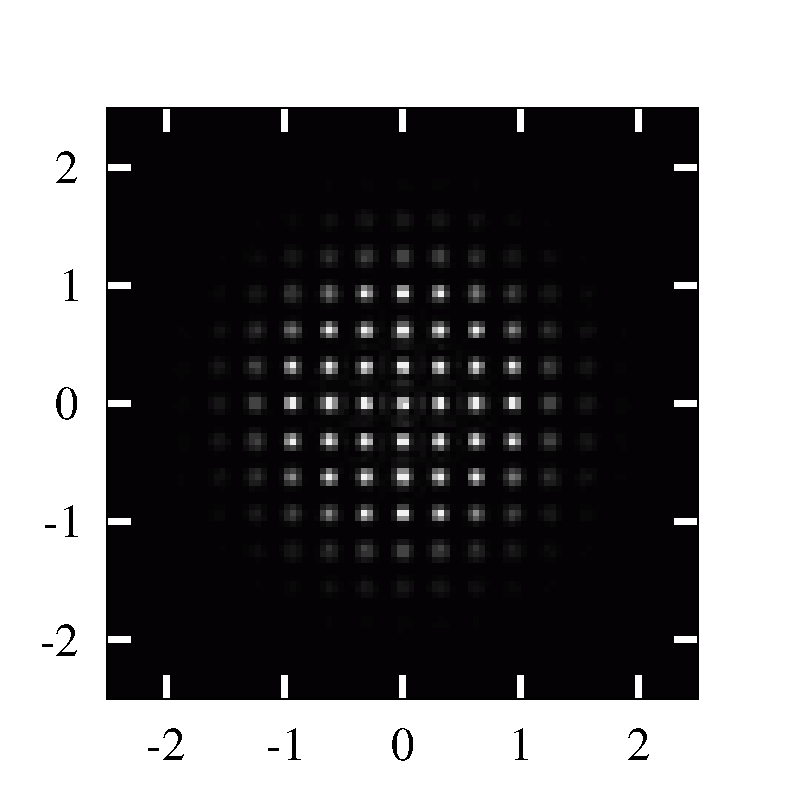
\includegraphics[width=0.95\linewidth]{beams/r_1000/outphase_norm} \\
            \footnotesize{Противофазный случай, \\ $z = 0.01$}}
        \end{minipage}
        \hfill
        \begin{minipage}{\minipagewidththree}
            \center{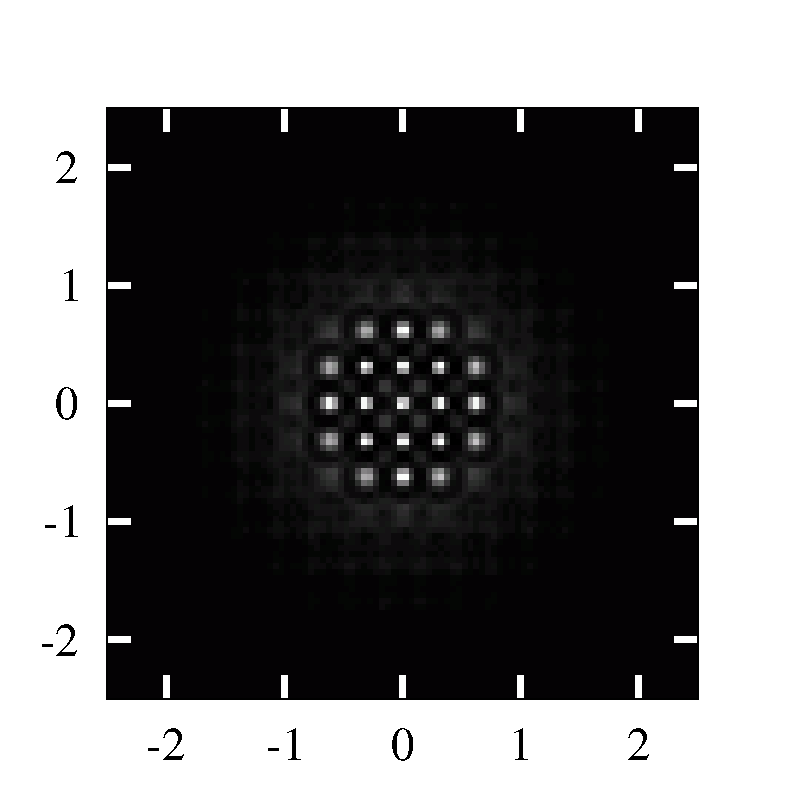
\includegraphics[width=0.95\linewidth]{beams/r_1000/inphase_norm} \\
            \footnotesize{Синфазный случай, \\ $z = 0.01$}}
        \end{minipage}
        \\[1ex]
        \caption{Филаментация отдельных пичков импульса при $R = 1000$. В этом случае мощность пучка превышает критическую в 66.5 раз,
                 а в центральном пичке содержится приблизительно 2 критические.}
        \label{fig:BeamsR1000}
    \end{center}
\end{figure}

%%%%%%%%%%%%%%%%%%%%%%%%%%%%%%%%%%%%%%%%

Как в случае противофазной модуляции, так и в случае синфазной возможно достичь такой
мощности исходного импульса, что критическая мощность будет превышена уже в~каждом из пичков в некоторой центральной области пучка.
В этом случае каждый из них будет образовывать филамент, как видно из рис. \ref{fig:BeamsR1000}.
Происходит независимая фокусировка нескольких пичков из центральной области пучка, тогда как пички на периферии испытывают дифракционное расплывание.
К сожалению, в рамках этой задачи было невозможно рассмотреть дальнейшее изменение пространственной конфигурации, так как из-за большой критической мощности
и разнице в расстоянии до нелинейного фокуса для различных пичков необходимость в учёте нестационарности и ионизации появляется до того, как периферийные пички начнут фокусироваться.


\subsection{Влияние случайных возмущений}

Все полученные выше результаты получены в предположении отсутствия шума. \mbox{Однако} лазерный пучок обычно имеет начальные флуктуации амплитуды и фазы.
Для моделирования этих возмущений можно использовать случайный амплитудный экран с заданной спектральной корреляционной функцией.

Радиус корреляции экрана, определяющий характерный размер
неоднородностей, обратно пропорционален полуширине $\kappa_0$ спектральной корреляционной
функции. Рассматривалась гауссова спектральная корреляционная функция, так как
она отражает случайные шумовые флуктуации на выходе лазерной системы:

\begin{equation}
    F_{\phi}(\kappa_x, \kappa_y) \sim \exp\left( -\frac{\kappa_x^2 + \kappa_y^2}{\kappa_0^2} \right)
\end{equation}

%%%%%%%%%%%%%%%%%%%%%%%%%%%%%%%%%%%%%%%%

\begin{figure}[h!]
    \begin{center}
        \begin{minipage}{\minipagewidththree}
            \center{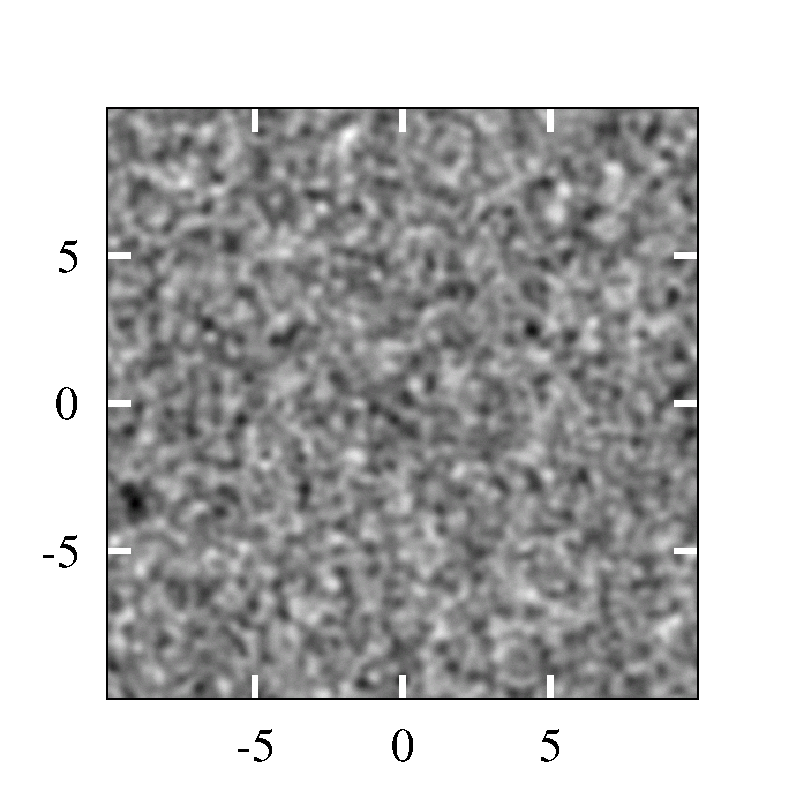
\includegraphics[width=0.95\linewidth]{beams/phasescreens/gauss_n8192_l10_r0dot5_real} \\
            \footnotesize{$r_{corr} = 0.5$}}
        \end{minipage}
        \hspace{\minipagewidthpadding}
        \begin{minipage}{\minipagewidththree}
            \center{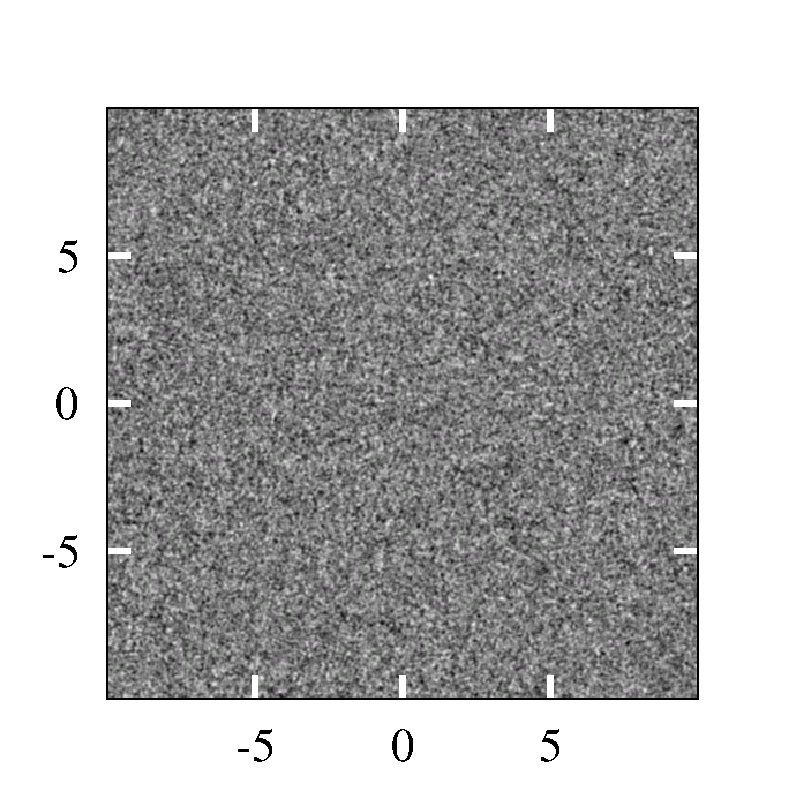
\includegraphics[width=0.95\linewidth]{beams/phasescreens/gauss_n8192_l10_r0dot125_real} \\
            \footnotesize{$r_{corr} = 0.125$}}
        \end{minipage}
        \\[1ex]
        \caption{Примеры случайных экранов, сгенерированных с использованием метода корреляционных функций.}
        \label{fig:BeamsPhasescreenExamples}
    \end{center}
\end{figure}

%%%%%%%%%%%%%%%%%%%%%%%%%%%%%%%%%%%%%%%%

На рис. \ref{fig:BeamsPhasescreenExamples} приведены примеры рассчитанных
по методу \cite{ShlenovKandidovTurbulence2004} экранов
(визуализировалась их действительная часть, используемая для~моделирования случайных амплитудных возмущений).                                      
Для моделирования использовался второй из приведённых экранов,
с $r_{corr} = 0.125$, при размере одного пичка в импульсе $a \simeq 0.3$, т.е. пространственный масштаб флуктуаций был меньше
характерного размера поперечной структуры импульса.

Для моделирования шума начальное распределение поля задавалось в виде:
\begin{equation}
    E(x, y, z = 0) = (1 + \beta \cdot \mathrm{Re} \phi(x, y)) \exp \left( -\frac{x^2 + y^2}{2 a^2}\right) \cos(\alpha_m x) \cos(\alpha_m y),
\end{equation}

\noindent где $\phi(x, y)$ "--- случайный экран с единичной дисперсией, а $\beta$ определяет относительную величину флуктуаций.

Проведённые вычисления показали, что при $\beta = 0.1$ эти возмущения заметно не~влияют на формирование
филамента. Так как на начальном этапе структура всё равно расплывается для образования одного
(в синфазном случае) или четырёх (в противофазном) импульсов, из которых и развивается филамент,
то эти флуктуации замазываются и~не~влияют на последующую филаментацию. 

%%%%%%%%%%%%%%%%%%%%%%%%%%%%%%%%%%%%%%%%

\newpage

\begin{figure}[h!]
    \begin{center}
        \begin{minipage}{\minipagewidththree}
            \center{\includegraphics[width=0.95\linewidth]{beams/outphase_phasescreen_0.5/out00000_norm} \\
            \footnotesize{$z = 0$}}
        \end{minipage}
        \hfill
        \begin{minipage}{\minipagewidththree}
            \center{\includegraphics[width=0.95\linewidth]{beams/outphase_phasescreen_0.5/out00100_norm} \\
            \footnotesize{$z = 0.1$}}
        \end{minipage}
        \hfill
        \begin{minipage}{\minipagewidththree}
            \center{\includegraphics[width=0.95\linewidth]{beams/outphase_phasescreen_0.5/out00200_norm} \\
            \footnotesize{$z = 0.2$}}
        \end{minipage}
        \\[2ex]
        \begin{minipage}{\minipagewidththree}
            \center{\includegraphics[width=0.95\linewidth]{beams/outphase_phasescreen_0.5/out00300_norm} \\
            \footnotesize{$z = 0.3$}}
        \end{minipage}
        \hfill
        \begin{minipage}{\minipagewidththree}
            \center{\includegraphics[width=0.95\linewidth]{beams/outphase_phasescreen_0.5/out00400_norm} \\
            \footnotesize{$z = 0.4$}}
        \end{minipage}
        \hfill
        \begin{minipage}{\minipagewidththree}
            \center{\includegraphics[width=0.95\linewidth]{beams/outphase_phasescreen_0.5/out00500_norm} \\
            \footnotesize{$z = 0.5$}}
        \end{minipage}
        \\[1ex]
        \caption{Формирование четырёх филаментов в противофазном случае для относительной амплитуды флуктуаций равной 0.5.}
        \label{fig:BeamsPhasescreenUsedBeta0.5}
    \end{center}
\end{figure}

%%%%%%%%%%%%%%%%%%%%%%%%%%%%%%%%%%%%%%%%

При увеличении величины $\beta$ до~0.5, когда исходное распределение интенсивности значительно изменяется (рис.~\ref{fig:BeamsPhasescreenUsedBeta0.5}),
можно получить небольшое изменение в поведении пучка, однако, в конечном счёте, на развитие филаментов это также не влияет.


\subsection{Выводы}

Рассмотрена возможность применения пучков с регулярной поперечной структурой для управления филаментацией
лазерного импульса.


Разработана программа, позволяющая исследовать распространение пучков в среде без дисперсии
с учётом дифракции и керровской нелинейности. Программа позволяет размещать расчётные данные
на нескольких вычислительных узлах вычислительного комплекса (небольшого кластера или суперкомпьютера),
что позволяет использовать её для сеток любого нужного размера.


Исследована филаментация гауссового пучка с регулярной поперечной структурой и~различными фазовыми соотношениями
между соседними элементами этой структуры. Проведена оценка критической мощности для такого пучка и показана её справедливость
для случая синфазного пучка. Обнаружено, что в случае противофазного пучка критическая мощность самофокусировки
примерно в 4 раза больше, чем в синфазном случае. Это связано с тем, что в этом случае исходный импульс образует четыре филамента.
Таким образом, если область значений мощности пучка, при которой в синфазном случае филамент образуется, а в противофазном -- нет.


Показано, что при одинаковых остальных параметрах в случае синфазной модуляции филамент
возникает значительно раньше, а в случае противофазной модуляции возникает четыре филамента,
разбегающиеся от оси распространения исходного импульса. Величину расхождения филаментов
можно оценивать на основе линейного уравнения, решение которого не требует больших вычислительных затрат.


Показано, что возможна ситуация, когда критическая мощность превышает критическую
для нескольких пичков в центральной части импульса, и тогда они независимо фокусируются, слабо взаимодействуя друг с другом.


Рассмотрено влияние случайных амплитудных возмущений начального пучка на~процесс возникновения
филамента и показано, что при относительной амплитуде шума $\beta \lesssim 0.5$ они значительно
не~влияют на процесс формирования филаментов.


Результаты проведённых исследований были доложены на конференциях \cite{Efimov2009} и \cite{ShlenovDergachevEfimov2009}.

